\documentclass[]{scrartcl}
\usepackage{enumerate}
\usepackage{graphicx}
\usepackage{rotating}

\title{CS 481 Lab 4}
\author{David Lochridge}

\begin{document}

\maketitle

\section*{Part 1}
\subsection*{1}
\begin{itemize}
\item[*] Overall execution time for all of the reads took 124813 milliseconds, making the cost per buffer read .00624 milliseconds, on average.
\item[*] The total time spent accessing the buffer was 77565 milliseconds.
\item[*] time reported that the time taken was 124.81 seconds, the user time was 108.35  seconds, and the system time was 87.30 seconds.
\end{itemize}
\subsection*{2}
\begin{itemize}
\item[*] Overall execution time for all of the exchanges was 267421 milliseconds, making the cost per exchange .01337 milliseconds, on average.
\item[*] The total time spent reading the buffer was 292580 milliseconds (146134 milliseconds for the parent and 146446 milliseconds for the child)
\item[*] time reported that the time taken was 267.42 seconds, the user time was 16.75 seconds, and the system time was 229.45 seconds.
\end{itemize}
\subsection*{3}
The measurements taken from within the program seem to be accurate for the overall measurement, but the amount of time spent reading and using CPU time do not seem to align, primarily in the multi-process program.
\subsection*{4}
The primary problem that I see with measuring using the time command is in the multi-process program, and calculating the total amount of CPU time used by both processes.

\section*{Part 2}
\subsection*{5}
I would expect that fread will outperform read, since it is doing buffering in the back-ground. In comparison to these two, I would expect that mmap()/memcpy() would
outperform both read and fread.
\subsection*{6}
For read() operations, I would expect performance to improve considerably as the stride
is increased.
\subsection*{7}
For fread() operations, I would expect performance to improve slightly as the stride is increased.
\subsection*{8}
For mmap() and memcpy(), I would expect the performance to increase more than the performance for read() operations increases.
\pagebreak

\begin{figure}
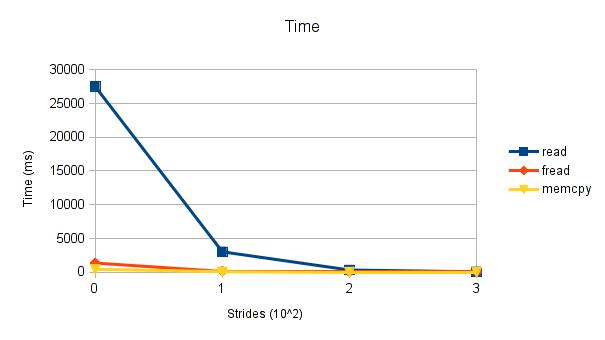
\includegraphics[width=0.5\textwidth]{Time.jpg}
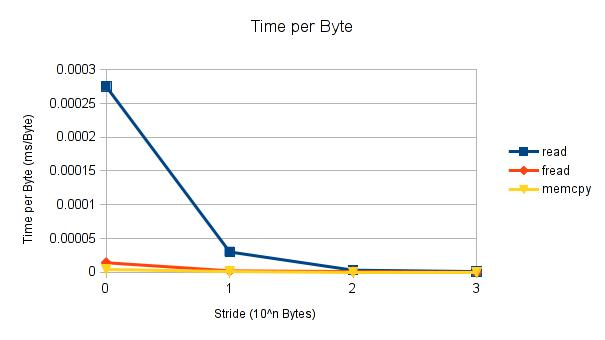
\includegraphics[width=0.5\textwidth]{TimePerByte.jpg}

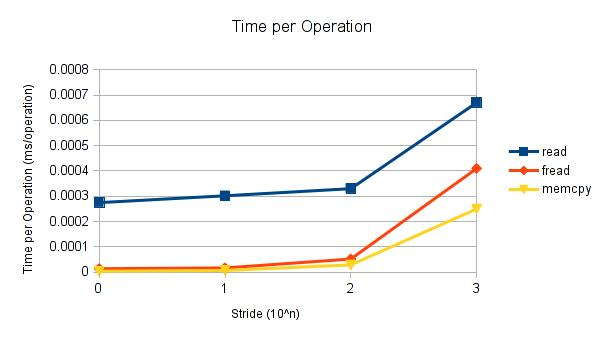
\includegraphics[width=0.5\textwidth]{TimePerOp.jpg}
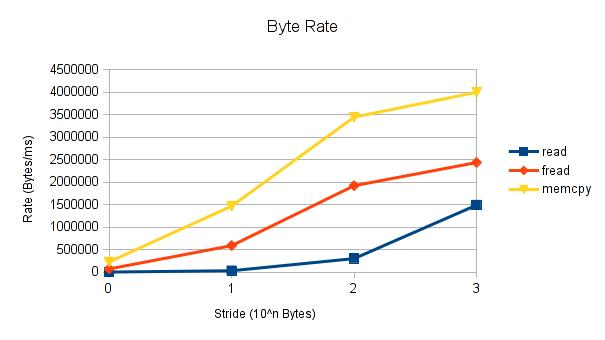
\includegraphics[width=0.5\textwidth]{BytePerTime.jpg}
\end{figure}

\section*{Conclusion}
As expected, fread outperformed read, and memcpy outperformed both read and fread. Read gained more and more performance as the strides got larger, while memcpy and fread started seeing diminishing returns with the size of stride. This likely happened because the buffers for both memcpy and fread were being used to their maximum ability after a stride somewhere between $10^2$ and $10^3$, leading to their diminished return.

The primary consideration for the performance increase from increased stride sizes is memory space. With less memory space, fread and memcpy would likely start performing worse than read, considering that the buffer would also be using some of the memory space, and requiring movement from memory to disk in the worst case.


\end{document}